\documentclass[acmsmall,screen,review,anonymous]{acmart}

\settopmatter{printacmref=false}
\setcopyright{none}
\renewcommand\footnotetextcopyrightpermission[1]{}

\usepackage{booktabs}
\usepackage{flafter}
\usepackage{multirow}
\usepackage{needspace}
\usepackage{tikz}
\usepackage{xspace}
\usetikzlibrary{arrows.meta,fit,positioning}

\newcommand{\model}{\textsc{Model}\xspace}
\newcommand{\prompttsg}{Prompt TSG\xspace}
\newcommand{\resultslot}{\mbox{\emph{Frozen-run results pending.}}}

\acmConference[FSE 2027]{The ACM International Conference on the Foundations
of Software Engineering}{July 12--16, 2027}{Shenzhen, China}
\acmYear{2027}
\copyrightyear{2027}

\begin{document}

\title{Prioritizing and Confirming Prompt-Side Security Interventions in LLM
Code Generation}

\author{Anonymous Author(s)}
\affiliation{%
  \institution{Anonymous Institution}
  \country{}
}

\begin{abstract}
Natural-language prompts are part of the security boundary of LLM code
generation: they can specify the required behavior while leaving validation,
authorization, trust boundaries, or safe-API constraints implicit. Existing
attribution and perturbation methods can expose influential text, yet they do
not by themselves turn that evidence into a task-preserving prompt
intervention with a confirmatory effect estimate. We present \model, a
three-stage framework that represents guard-independent task/security context,
prioritizes one-feature intervention hypotheses with structure-constrained
FCI, and tests frozen multi-realization prompt policies on held-out tasks. The
discovery stage combines graph-derived variables, typed background knowledge,
and semantic-task-cluster bootstrap stability while preserving PAG
uncertainty. The confirmation stage freezes complete four-arm prompt bundles
before blocked random assignment and estimates semantic-task-clustered
assigned-arm intent-to-treat effects on oracle-evaluable secure-code yield. A
shared candidate universe supports controlled comparisons among causal,
associational, predictive, expert, and random selectors. \resultslot
\end{abstract}

\begin{CCSXML}
<ccs2012>
 <concept>
  <concept_id>10011007.10011074.10011099</concept_id>
  <concept_desc>Software and its engineering~Software safety</concept_desc>
  <concept_significance>500</concept_significance>
 </concept>
 <concept>
  <concept_id>10002978.10003029.10011703</concept_id>
  <concept_desc>Security and privacy~Software security engineering</concept_desc>
  <concept_significance>500</concept_significance>
 </concept>
</ccs2012>
\end{CCSXML}

\ccsdesc[500]{Software and its engineering~Software safety}
\ccsdesc[500]{Security and privacy~Software security engineering}
\keywords{large language models, code generation, software security, causal
discovery, randomized experiments, prompt analysis}

\maketitle
\raggedbottom

\section{Introduction}

Natural-language prompts now participate directly in the security boundary of
code generation. They often specify what a program should do while leaving
validation, authorization, trust boundaries, or safe-API constraints implicit.
Studies of AI-assisted code generation show that functional-looking outputs
can still contain security weaknesses and that developers may overestimate the
security of assisted solutions~\cite{pearce2022copilot,perry2023assistants}.
The practical question is therefore not only which prompt text matters, but
which missing or weakly scoped requirement can be edited without changing the
programming task.

Feature attribution, concept-based interpretation, and rationale evaluation
offer complementary views of model
behavior~\cite{sundararajan2017integrated,kim2018tcav,lundberg2017shap,deyoung2020eraser},
but importance or plausibility alone does not identify the effect of an
editable prompt requirement. Perturbations can further reveal behavioral
sensitivity to changed text, yet an unconstrained change may alter task
semantics, presentation, and security content together. These signals are
valuable evidence sources, but they do not by themselves supply a
task-preserving intervention or a confirmatory effect estimate.

The missing link is a reproducible progression from \emph{representation}, to
\emph{hypothesis}, to \emph{effect}. Free-form requirements must first become
typed, scoped, and editable prompt-side factors. Observational relations among
those factors must then retain their uncertainty and remain stable across task
clusters. Finally, the selected hypothesis and its intervention protocol must
be fixed before held-out outcomes exist, so that confirmation estimates the
effect of assignment rather than selecting cases in which the intended edit
happened to succeed.

\model provides this progression in three stages.
\textbf{Security-Aware Prompt Representation} separates an immutable
task/security context query from one catalog-bound editable feature.
\textbf{Stability-Guided Causal Prioritization} combines structure-derived
constraints, FCI, and semantic-task-cluster stability to rank candidates while
preserving PAG uncertainty.
\textbf{Randomized Policy Confirmation} freezes a finite distribution of
task-independent realizations, constructs complete task-specific four-arm
bundles, randomizes them on held-out tasks, and estimates assigned-arm
intent-to-treat effects. A shared-universe selector comparison and an explicit
candidate-to-policy bridge make both prioritization and confirmation auditable.

This paper makes the following contributions:

\begin{itemize}
  \item \textbf{Security-aware prompt representation.} A typed, catalog-bound
  representation converts free-form requirements into guard-independent
  contexts and scoped, editable security features.
  \item \textbf{Budgeted intervention prioritization.} Typed background
  knowledge, FCI, and semantic-task-cluster stability rank a frozen candidate
  universe alongside associational, predictive, expert, and random selectors.
  \item \textbf{Randomized policy confirmation.} Multi-realization prompt
  policies and held-out blocked randomization produce hypothesis-specific
  assigned-arm ITT evidence without conditioning on realized edit success.
  \item \textbf{Provenance-complete evidence accounting.} An explicit bridge
  records context eligibility, policy realization, protocolization,
  randomization, and confirmation without upgrading exploratory artifacts.
\end{itemize}

\section{Motivating Example and Problem Formulation}

\subsection{An Editable Prompt-Side Security Factor}

Consider a security-neutral request to implement
\texttt{read\_report(base\_dir, user\_path)} and return the requested UTF-8
report. The request fixes the task but leaves path confinement implicit. A
target-specific variant can require resolving and normalizing the path under
\texttt{base\_dir} and rejecting any resolution outside that directory. A
no-op variant preserves the original security semantics, a length-matched
placebo changes presentation only, and a generic-control variant requests
secure coding without naming path confinement. Together, these controls
isolate rewrite, presentation/length, and generic security-cue effects,
respectively. This illustrative example defines an intervention question; it
does not report a generated program or an effect.

\subsection{Units, Outcomes, and Claim Scope}

Let a generation unit be indexed by semantic task cluster $c$, task instance
$i$, hypothesis $h$, realization $r$, prompt arm $a$, model $m$, and request
randomness slot $s$:

\[
  u = (c,i,h,r,a,m,s).
\]

Tasks are partitioned before model-based discovery into disjoint discovery and
confirmation pools. The discovery pool supports observational hypothesis
formation; the held-out confirmation pool supports prompt construction,
randomized assignment, code generation, and effect estimation. No semantic
task cluster crosses this boundary. The highest resampling unit is
\texttt{semantic\_task\_cluster\_id}; every descendant task instance,
hypothesis, model, arm, realization, and request slot moves with its cluster.

The primary analysis estimates semantic-task-clustered assigned-arm ITT on
\emph{oracle-evaluable secure-code yield} for every committed assignment.
Secure-and-functional joint success is a key practical secondary outcome, not
a condition for the primary security effect. Valid terminal non-successes
remain in the assigned-arm denominator; a missing or corrupt required producer
instead blocks publication and requires deterministic replay of the same
assignment manifest.

$W$ contains approved pre-treatment task metadata, $X^0$ contains natural
Prompt TSG feature queries, and $Y^0$ contains independently committed
discovery outcomes. A non-editable context query $C_q$ scopes one actionable
feature $f$. Randomized arm $A$ is the confirmation treatment;
post-intervention $X^{A,R}$ is a separately extracted projection diagnostic
and never replaces $A$ in the ITT estimator. Model identity remains an analysis
coordinate and provenance field.

The \prompttsg defines typed prompt structure and the editable queries supplied
to discovery, while the PAG preserves FCI uncertainty over learned relations.
Generated code is used only by the independent security Oracle and functional
checker. Observational paths therefore form hypotheses, and confirmatory claims
are limited to task-clustered assigned-arm effects of frozen prompt
interventions on held-out tasks within their hypothesis, target, operation,
model, and CWE scopes.

\section{Security-Aware Prompt Representation}

\model first turns a programming request into factors that can be named,
scoped, and edited while preserving the requested task. This makes an implicit
security requirement available as an intervention target and keeps task
behavior and surface presentation separately auditable.
Figure~\ref{fig:overview} previews this route from representation to hypothesis
formation and confirmation, with disjoint discover and held-out splits
separated by a pre-confirmation freeze.

\begin{figure}[t]
  \centering
  \resizebox{\linewidth}{!}{%
    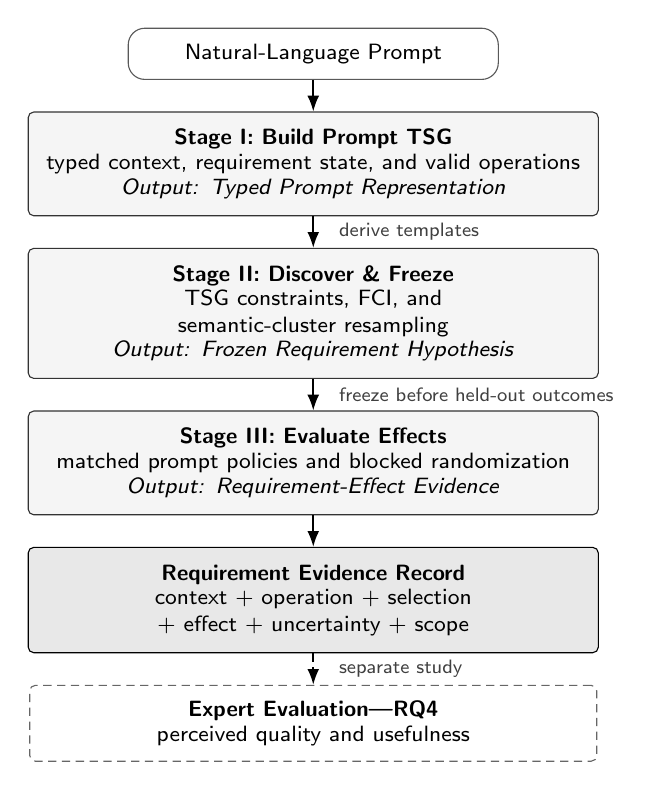
\begin{tikzpicture}[
  font=\sffamily\footnotesize,
  input/.style={draw=black!65,rounded corners=6pt,align=center,
    minimum height=6.5mm,minimum width=47mm,fill=white},
  stage/.style={draw=black!80,rounded corners=2pt,align=center,
    text width=68mm,minimum height=12mm,fill=black!4,inner sep=2.2mm},
  record/.style={draw=black,rounded corners=2pt,align=center,
    text width=68mm,minimum height=11mm,fill=black!9,inner sep=2.2mm},
  downstream/.style={draw=black!60,densely dashed,rounded corners=2pt,
    align=center,text width=68mm,minimum height=9mm,fill=white,inner sep=2mm},
  flow/.style={-{Latex[length=2mm]},semithick},
  downstreamflow/.style={-{Latex[length=2mm]},semithick,densely dashed},
  note/.style={font=\sffamily\scriptsize,align=left,text=black!75}
]
  \node[input] (prompt) {Natural-Language Prompt};

  \node[stage,below=4mm of prompt] (repr) {
    \textbf{Stage I: Build Prompt TSG}\\[-0.2mm]
    typed context, requirement state, and valid operations\\[-0.2mm]
    \textit{Output: Typed Prompt Representation}};

  \node[stage,below=4mm of repr] (select) {
    \textbf{Stage II: Discover \& Freeze}\\[-0.2mm]
    TSG constraints, FCI, and semantic-cluster resampling\\[-0.2mm]
    \textit{Output: Frozen Requirement Hypothesis}};

  \node[stage,below=4mm of select] (evaluate) {
    \textbf{Stage III: Evaluate Effects}\\[-0.2mm]
    matched prompt policies and blocked randomization\\[-0.2mm]
    \textit{Output: Requirement-Effect Evidence}};

  \node[record,below=4mm of evaluate] (record) {
    \textbf{Requirement Evidence Record}\\[-0.2mm]
    context + operation + selection + effect + uncertainty + scope};

  \node[downstream,below=4mm of record] (expert) {
    \textbf{Expert Evaluation---RQ4}\\[-0.2mm]
    perceived quality and usefulness};

  \draw[flow] (prompt) -- (repr);
  \draw[flow] (repr) -- node[note,right=2mm] {derive templates} (select);
  \draw[flow] (select) -- node[note,right=2mm] {freeze before held-out outcomes} (evaluate);
  \draw[flow] (evaluate) -- (record);
  \draw[downstreamflow] (record) -- node[note,right=2mm] {separate study} (expert);
\end{tikzpicture}

  }
  \caption{\model converts prompt semantics into frozen intervention policies
  and evaluates their security effects on held-out tasks. Prompt TSG edges provide
  typed structure rather than causal conclusions; generated code enters only
  the independent Oracle and functional-evaluation path in the confirmation
  stage.}
  \Description{Three-stage \model workflow. The discover split contains
  security-aware prompt representation and stability-guided observational
  prioritization. A policy-freeze boundary separates it from randomized
  confirmation on held-out tasks using multi-realization prompt arms, block
  randomization, generated-code evaluation, and assigned-arm ITT estimation.}
  \label{fig:overview}
\end{figure}

\subsection{Typed Prompt Semantics}

For each prompt, \model separates three semantic families. Task-function
factors describe required operations and functional constraints; safety-control
factors describe guards, trust boundaries, assets, and security requirements;
and presentation-control factors describe wording and formatting used for
matched controls.

We encode these families in a bounded, typed task-security graph over the
prompt, which we call the \prompttsg.
Its relations encode prompt task/security structure---for example, that a
validation requirement is scoped to a sensitive input---not causal edges.
Every intervenable identity, scope, state, graph template, query, and permitted
ADD/REMOVE operation comes from an immutable versioned catalog. Extracted facts
must satisfy catalog closure and carry exact evidence spans into the prompt.
Deterministic validation checks those spans, family compatibility, and
duplicate or conflicting identities. Accepted records undergo canonical
node/edge identification, ordering, serialization, round-trip validation, and
digesting. The states \textsc{present}, \textsc{absent},
\textsc{not-applicable}, and \textsc{unresolved} remain distinct.

The intervention language distinguishes a non-editable context-query
specification $C_q$ from an actionable-feature specification $f$.
The former expresses guard-independent applicability, such as an untrusted
input reaching a shell operation; the latter names exactly one actionable
feature that an ADD or REMOVE policy may edit. A confirmable composite maps one
$C_q$ to exactly one actionable feature. Task operations, sources, sinks, APIs,
trust boundaries, and flow motifs remain context or effect-modifier
coordinates and are never silently edited to make a candidate actionable.

\subsection{Run-Locked Extraction}

\model supports three ways to build the same catalog-bound representation. An
LLM can emit catalog-bound semantic facts for deterministic graph construction
(\path{LLM_FACTS_V1}); it can instead emit a catalog-bound typed graph for
strict validation and canonicalization
(\path{LLM_DIRECT_GRAPH_V1}); or the reviewed finite matcher and templates
can construct the graph deterministically
(\path{DETERMINISTIC_CATALOG_V1}). Before processing any prompt, a run
selects exactly one backend and keeps it fixed throughout; per-prompt switching
and outcome-guided candidate selection are prohibited.

The extraction policy fixes provider, model, template, catalog, schema,
decoding, and request policy. The extractor treats the prompt as inert data and
is isolated from the target, arm, generated code, Oracle records, and outcomes.
It emits one semantic candidate. A transport failure may resend identical
request bytes, but the retry may not change semantic content or choose among
candidates for a favorable output.

\subsection{Local Causal Variables}

\model builds a local table for each configured CWE/security scope and model.
$W$ contains an approved minimal set of pre-treatment task metadata, $X^0$
contains non-deterministic natural-Prompt TSG queries, and $Y^0$ contains
independently committed discovery outcomes. Model identity remains an analysis
coordinate and provenance field. Raw text, generated code, code structure,
Oracle finding text, assigned arm $A$, and post-intervention $X^{A,R}$ are not
observational-table variables: generated code enters only the independent
Oracle and functional evaluator that produce $Y^0$.

\section{Stability-Guided Observational Prioritization}

The second stage converts prompt-side variables into a bounded set of
intervention candidates. It combines type-derived exclusions with FCI evidence
that preserves endpoint uncertainty, then tests whether candidate relations
remain stable when whole semantic task clusters are resampled. FCI is one
budgeted selector; held-out randomization, not a PAG endpoint, identifies the
prompt-policy effect.

\subsection{TSG-Derived Constraints}

The Prompt TSG supplies variables, background knowledge, and edge constraints;
it does not supply learned causal edges. Temporal tiers prohibit outcomes from
causing pre-treatment metadata or prompt factors. Catalog types define
family- and scope-specific forbidden directions, and typed adjacency
restrictions exclude semantically impossible local relations. These rules may
forbid both directions of an adjacency, but they never require a
feature--outcome edge or any edge on the possible path being tested. \model
persists the exact tiers, forbidden pairs, typed adjacency matrix, variable
order, and background-knowledge digest and validates every learned PAG against
them.

\subsection{FCI and Semantic-Cluster Stability}

The minimum backend is the established causal-learn implementation of
FCI~\cite{spirtes1995fci,zheng2024causallearn}. Its PAG output preserves
endpoint uncertainty under latent-variable assumptions rather than selecting a
single convenient orientation~\cite{zhang2008ancestral}. The run locks the
G-square conditional-independence test, variable order, significance level,
depth and path bounds, backend version, and background knowledge.

The fixed-reference analysis selects one frozen request-randomness slot per
task. The two-level analysis resamples \texttt{semantic\_task\_cluster\_id}
and then selects one frozen request slot inside each sampled task occurrence.
A separately frozen multi-slot sensitivity aggregates slots at task level
without passing fractional pseudo-categories to G-square. None treats repeated
generations, task instances, or rows as independent clusters.

Candidate extraction retains PAG endpoint marks and scores permitted
feature--outcome adjacency, endpoint-compatible possible ancestry, or the same
relation within the frozen $C_q$-eligible population. Simultaneously authored
Prompt features occupy one temporal tier: their within-tier endpoints are not
interpreted as security mechanisms or mediation. \model applies a fixed
top-$K$ budget and deterministic ordering rather than claiming recovery of a
unique DAG.

\subsection{Hypothesis Freeze}

Before any selector runs, one \texttt{CandidateUniverseManifest} freezes
skeletons $\widetilde h=(C_q,f,a,\mathcal Q_h,Y)$ and their common information
budget. After all rankings are frozen, the unique top-$K$ union crosses one
selector-invariant, outcome-blind bridge. A successful bridge produces
$h=(C_q,f,a,Q_h,Y)$, binding one non-actionable context, one actionable
feature, one atomic operation, a finite realization distribution, and one
outcome. Its record also binds CWE/model scope, reference PAG endpoints,
semantic-cluster support, expected direction, and the table, catalog,
extractor, selector, CI-test, and background-knowledge provenance.

This hypothesis freeze is committed before any confirmation variant,
assignment, generated code, or outcome exists. Held-out evidence may classify
a frozen hypothesis, but it cannot add, remove, rerank, remap, or rewrite one.
An empty, bridge-failed, or protocolization-failed selector slot remains a zero
in the original budget denominator.

\section{Causal Effect Confirmation}

The third stage turns each frozen hypothesis into a family-valid randomized
experiment on held-out tasks. Typed variants and their controls are completed
before assignment, and analysis estimates the effect of assigned prompt roles
without selecting cases by realized edit success.

\subsection{Typed Intervention Protocols}

A \texttt{TargetSpec} binds the feature family and catalog identity, ADD or
REMOVE, source prompt role, and exact counterpart requirements. ADD requires
an applicable, resolved \textsc{absent} source state. REMOVE requires a
provenance-bound \textsc{present} clause and a pre-attested, task-preserving
neutral counterpart. Execution is text-native or graph-native and uses either
a deterministic renderer or a locked LLM executor; the run fixes this choice
and its complete provenance.

Four-arm protocols are specific to Safety ADD and Safety REMOVE:

\begin{itemize}
  \item Safety ADD uses \path{TARGET_PATCH}, \path{NOOP_REWRITE},
  \path{LENGTH_MATCHED_PLACEBO}, and
  \path{GENERIC_SECURITY_REMINDER}.
  \item Safety REMOVE uses \path{TARGET_REMOVE}, \path{NOOP_RETAIN},
  \path{LENGTH_MATCHED_SHAM_EDIT}, and
  \path{GENERIC_SECURITY_REPLACEMENT}.
\end{itemize}

ADD and REMOVE remain separate candidate slots, hypotheses, protocols,
contrasts, multiplicity coordinates, and evidence. REMOVE may only restore an
attested neutral counterpart and never inserts an unsafe request; ADD and
REMOVE therefore cannot be combined in one confirmable hypothesis.

Other families retain family-specific protocols. Task-function ADD/REMOVE
requires target, no-op, and length-matched placebo roles; a fourth active
control is permitted only with a reviewed catalog entry and independent
functional outcome. Presentation experiments use target and no-op plus an
optional matched presentation control and serve as negative controls.

Each arm has an explicit \texttt{AllowedDelta} that bounds its declared target
or control change and fixes protected task, safety, and presentation
projections. Exact source/counterpart provenance and the
\texttt{SecurityNeutralPromptInvariant} ensure that no variant claims a
vulnerability, requests unsafe behavior, or reveals an expected Oracle label
or effect direction.

\subsection{Variant Freeze and Block Randomization}

For each $h$, the protocol first freezes a finite task-independent realization
set and probabilities $Q_h$. For every eligible task and every realization,
one task-specific bundle contains all four arm texts and exact digests. Every
candidate arm is independently re-extracted with the run-locked Prompt
extractor while it is blind to the arm role and target. Before assignment, hard
gates validate schema and catalog integrity, exact evidence and provenance,
canonical round trips, security-neutral task preservation, context/task/non-
target invariance, the arm-specific \texttt{AllowedDelta}, and absence of
downstream information. A task enters the common-support population only when
every required arm and realization passes before outcomes exist; failed
realizations are never deleted or renormalized.

Target change, semantic compliance, and permissible non-target drift are
recorded during this arm-blind validation as intervention-realization
diagnostics. They
do not decide the hard-gate result, and \texttt{target\_changed}, semantic
compliance, and non-target drift never filter the primary assigned-arm ITT
denominator. If one arm fails a hard gate, the complete task--hypothesis bundle
is reported as a pre-randomization exclusion and receives no assignment.

Within each complete frozen block, a manifested deterministic RNG assigns
request-randomness slots to a balanced permutation of the protocol's finite arm
roles. The canonical block binds semantic cluster, task instance, hypothesis,
target, global realization specification, task realization bundle, model, and
arm protocol. The assignment manifest additionally binds prompt variant,
nullable provider seed, model parameters, RNG identity, request order, and
request ID before generation. Mutation of any canonical coordinate changes the
block identity, and provider execution order cannot alter treatment.

\subsection{Outcomes and Assigned-Arm ITT}

Generated code enters only the independent, versioned security Oracle and
functional evaluator. We decompose code production and Oracle support as
$Y_C$ and $Y_E$. The primary oracle-evaluable secure-code yield is
$Y_CY_E I(\text{Oracle secure})$; secure-and-functional joint success further
requires the frozen functional check to pass and is the key practical
secondary outcome. A valid terminal generation failure or syntactically
invalid result has $Y_C=0,Y_E=0$; valid but Oracle-unsupported or unknown code
has $Y_C=1,Y_E=0$. These remain observed assigned-arm outcomes under the
frozen encoding. Missing, corrupt, or unavailable required producer evidence
is not encoded as an outcome; it blocks publication and triggers deterministic
replay of the same manifest.

For frozen hypothesis $h$, target $q$, operation $o$, model $m$, and outcome
$Y$, the primary contrast is the hypothesis-specific target-minus-no-op
assigned-arm ITT risk difference

\[
  \Delta^{\mathrm{ITT}}_{h,q,o,m}
  = \mathbb{E}[Y \mid A=\mathrm{target}]
  - \mathbb{E}[Y \mid A=\mathrm{no\mbox{-}op}].
\]

Every committed randomized assignment enters the denominator under its
assigned role. Point estimates average over the frozen task population and
realization distribution $Q_h$. Uncertainty resamples semantic task clusters
and carries all descendant hypotheses, models, arms, realizations, and request
slots together. Simultaneous intervals follow the frozen hypothesis/model/
contrast family. Target-minus-placebo and, where family-valid,
target-minus-generic-control contrasts assess specificity. Effects remain
separate by hypothesis, target, operation, model, and CWE unless another
estimand was approved in advance. Task improvement, harm, and tie rates remain
descriptive diagnostics, not individual causal flips or substitutes for ITT.

\subsection{Evidence Levels}

\model uses the prospective evidence levels below:

\begin{enumerate}
  \item \textbf{Observational Candidate}: a discover-split stable possible path
  frozen before confirmation, without a causal confirmation claim.
  \item \textbf{Randomized Policy Effect}: the preregistered
  target-minus-no-op ITT follows the frozen expected direction, meets the
  independent-task requirement, and has a multiplicity-adjusted interval
  excluding zero with complete provenance.
  \item \textbf{Target-Specific Policy Effect}: a randomized effect also supported by
  the preregistered target-minus-placebo and, where family-valid,
  target-minus-generic contrasts.
  \item \textbf{Realization-Robust Policy Effect}: the average policy effect
  is confirmed and all frozen direction, equivalence, interaction, and
  leave-one-realization-out conditions hold simultaneously.
  \item \textbf{Cross-Model Replication}: separately estimated model effects
  meet the frozen replication rule without creating a pooled universal effect.
  \item \textbf{Bidirectional Support}: separate ADD and REMOVE protocols
  independently confirm opposite expected directions for the same feature.
  \item \textbf{Directionally Consistent but Inconclusive}: the point estimate
  follows the frozen direction but its adjusted interval includes zero or
  independent-task support is insufficient.
  \item \textbf{Null / Conflicting / Non-Evaluable}: the preregistered analysis
  respectively detects no effect, estimates the opposite direction, or cannot
  publish an effect because no valid randomization universe or required
  infrastructure/provenance exists.
\end{enumerate}

Valid post-assignment terminal non-successes remain assigned data and do not
create a non-evaluable result. Discovery, demo, and smoke-test artifacts cannot
be promoted to confirmatory evidence.

\section{Evaluation Design and Results}

All computational methods receive the same discover and confirm task
manifests, model and request-randomness policy, independent Oracle and
functional contract, candidate budget, family-valid intervention protocol,
randomization, outcome encoding, semantic-cluster uncertainty, and
multiplicity policy. Candidate universes, selector scores and ranks, native
candidates, mappings, expected directions, and realization policies are frozen
before confirm outcomes exist.

Discovery uses the discover split, and randomized confirmation uses held-out
confirm tasks. The primary confirmatory analysis is hypothesis- and
model-specific semantic-task-clustered assigned-arm ITT on oracle-evaluable
secure-code yield. Secure-and-functional joint success is the key practical
secondary outcome. Every
committed assignment remains in its assigned-arm denominator;
\texttt{target\_changed}, semantic compliance, and non-target drift are
diagnostics rather than filters.

Throughout the tables, \texttt{--} marks a result slot awaiting
provenance-verified frozen-run or study backfill; it denotes neither zero, not
applicable, nor observed missingness.

\subsection{RQ1: Held-Out Intervention Prioritization}

\textbf{RQ1. How effectively can different methods prioritize prompt
interventions that generalize to held-out tasks?}

The primary selector-only comparison gives TSG-constrained FCI,
preregistered association, regularized prediction, blinded expert ranking, and
seeded random ranking the same shared candidate universe, information budget,
and $K$ slots. The unique union of their top-$K$ skeletons crosses the common
bridge once and each resulting hypothesis is randomized once; duplicate
selector references reuse that evidence. Empty, bridge-failed, and
protocolization-failed slots remain zeroes in denominator $K$. The primary
endpoint is strict confirmed yield at $K$, accompanied by simultaneous paired
selector-utility differences. Rankings remain conditional on the frozen
discover split; held-out outcomes neither rerank selectors nor replace failed
slots.

A separate native-system track provides secondary end-to-end evidence using
the fixed funnel

\[
K \rightarrow N_{\mathrm{native}} \rightarrow N_{\mathrm{mapped}}
\rightarrow N_{\mathrm{protocol}} \rightarrow N_{\mathrm{randomized}}
\rightarrow N_{\mathrm{confirmed}}.
\]

That track measures system compatibility rather than pure selector
superiority. Conditional mapping coverage and mapped yield at $K$ are bridge
diagnostics; native funnel results cannot replace the shared-universe primary
comparison. For every frozen method/slot hypothesis, the evidence report
retains target and operation, target-minus-no-op ITT, simultaneous status,
independent semantic-cluster and arm counts, and preregistered specificity
contrasts.

\begin{table}[H]
  \centering
  \small
  \caption{RQ1 shared-universe selector results. Panel A retains every frozen
  budget slot through confirmation. Panel B reports the corresponding yields;
  strict confirmed yield at $K$ is primary. FCI, association, prediction,
  expert, and random rankings use identical candidate and information
  budgets.}
  \label{tab:rq1}
  \begin{tabular}{lrrrrrr}
    \toprule
    \multicolumn{7}{l}{\textit{Panel A: Frozen-slot funnel}} \\
    \midrule
    Selector & $K$ & Selected & Bridged & Protocol & Rand. & Conf. \\
    \midrule
    TSG-constrained FCI & -- & -- & -- & -- & -- & -- \\
    Association & -- & -- & -- & -- & -- & -- \\
    Regularized prediction & -- & -- & -- & -- & -- & -- \\
    Blinded expert & -- & -- & -- & -- & -- & -- \\
    Seeded random & -- & -- & -- & -- & -- & -- \\
    \bottomrule
  \end{tabular}

  \medskip
  \begin{tabular}{lrrrrr}
    \toprule
    \multicolumn{6}{l}{\textit{Panel B: Derived yields}} \\
    \midrule
    Metric & FCI & Assoc. & Predict. & Expert & Random \\
    \midrule
    Selected / $K$ & -- & -- & -- & -- & -- \\
    Bridged / $K$ & -- & -- & -- & -- & -- \\
    Protocol / $K$ & -- & -- & -- & -- & -- \\
    Unique-union share & -- & -- & -- & -- & -- \\
    Block-freeze coverage & -- & -- & -- & -- & -- \\
    Randomized / $K$ & -- & -- & -- & -- & -- \\
    Strict confirmed yield / $K$ & -- & -- & -- & -- & -- \\
    Confirmed / Randomized & -- & -- & -- & -- & -- \\
    \bottomrule
  \end{tabular}
\end{table}

\begin{table}[H]
  \centering
  \small
  \caption{RQ1 hypothesis and paired-selector evidence. The frozen RQ1
  manifest binds selector/slot references to one shared randomized hypothesis
  estimate. Paired utility intervals resample top-level semantic clusters and
  never rerun discovery.}
  \label{tab:rq1-evidence}
  \begin{tabular}{llllrr}
    \toprule
    Selector/slot & Hyp.\ ID & Frozen target & Op. & ITT RD & Interval \\
    \midrule
    \multicolumn{6}{c}{\emph{Rows are populated only from the
    provenance-verified frozen RQ1 manifest}} \\
    \bottomrule
  \end{tabular}

  \medskip
  \begin{tabular}{llrrl}
    \toprule
    Selector pair & Utility diff. & Simult.\ interval & Status & Shared slots \\
    \midrule
    \multicolumn{5}{c}{\emph{Continued fields for the same frozen rows}} \\
    \bottomrule
  \end{tabular}
\end{table}

\subsection{RQ2: Representation and Prioritization Contribution}

\textbf{RQ2. How do \model's structured representation and causal
prioritization contribute to successful intervention selection?}

RQ2 separates two questions that require different controls. The selector-only
track reuses RQ1's direct-plus-context universe and holds every candidate,
eligibility rule, outcome, realization policy, and information budget fixed
while changing only the selector. Its FCI-versus-baseline comparisons therefore
isolate prioritization under a shared universe.

The representation comparison contrasts a direct-actionable-feature universe
with a direct-plus-context universe. Because the candidate identities and
eligible populations can differ, this is an end-to-end comparison, not a pure
selector comparison. Both universes use the same frozen budget, bridge,
confirmation protocol, and outcome construction, and report candidate
coverage, protocolization, strict confirmed yield at $K$, and the distribution
of hypothesis-specific effects. No selected hypotheses are pooled into an
unapproved cross-hypothesis ATE.

\begin{table}[H]
  \centering
  \small
  \caption{RQ2 separates selector-only and representation evidence. Panel A
  reports shared direct-plus-context-universe selector yields. Panel B compares
  direct and direct-plus-context universes end-to-end without interpreting the
  result as pure selector superiority.}
  \label{tab:rq2}
  \begin{tabular}{lrrrrr}
    \toprule
    \multicolumn{6}{l}{\textit{Panel A: Selector-only outcomes}} \\
    \midrule
    Metric & FCI & Assoc. & Predict. & Expert & Random \\
    \midrule
    Selected / $K$ & -- & -- & -- & -- & -- \\
    Bridged / $K$ & -- & -- & -- & -- & -- \\
    Protocol / $K$ & -- & -- & -- & -- & -- \\
    Block-freeze coverage & -- & -- & -- & -- & -- \\
    Randomized / $K$ & -- & -- & -- & -- & -- \\
    Strict confirmed yield / $K$ & -- & -- & -- & -- & -- \\
    Paired utility vs. FCI & -- & -- & -- & -- & -- \\
    Simultaneous status & -- & -- & -- & -- & -- \\
    \bottomrule
  \end{tabular}

  \medskip
  \begin{tabular}{lrrrrr}
    \toprule
    \multicolumn{6}{l}{\textit{Panel B: Representation end-to-end outcomes}} \\
    \midrule
    Universe & Candidates & Coverage & Protocol & Rand. & Strict yield / $K$ \\
    \midrule
    Direct features & -- & -- & -- & -- & -- \\
    Direct + context & -- & -- & -- & -- & -- \\
    \bottomrule
  \end{tabular}
\end{table}

\begin{table}[H]
  \centering
  \small
  \caption{RQ2 hypothesis-specific evidence. Selector-only rows retain one
  shared-universe identity; representation rows retain their distinct universe
  identity. Every row reports target-minus-no-op ITT and its simultaneous
  status without cross-hypothesis pooling.}
  \label{tab:rq2-evidence}
  \begin{tabular}{llllrr}
    \toprule
    Track/universe & Hyp.\ ID & Frozen target & Op. & ITT RD & Interval \\
    \midrule
    \multicolumn{6}{c}{\emph{Rows are populated only from the
    provenance-verified frozen RQ2 manifest}} \\
    \bottomrule
  \end{tabular}

  \medskip
  \begin{tabular}{llrrl}
    \toprule
    Hyp.\ ID & Adj.\ status & Indep.\ clusters & Arm counts & Specificity contrasts \\
    \midrule
    \multicolumn{5}{c}{\emph{Continued fields for the same frozen rows}} \\
    \bottomrule
  \end{tabular}
\end{table}

\Needspace{8\baselineskip}
\subsection{RQ3: Security Intervention Effects}

\textbf{RQ3. Which prompt-side security interventions reliably improve secure
code generation?}

RQ3 estimates context-conditioned, model-specific, multi-realization policy
effects for the frozen security targets. The primary outcome is
oracle-evaluable secure-code yield; secure-and-functional joint success is the
key practical secondary outcome. Code validity, Oracle support, unknowns,
terminal no-code rates, and secure-yield bounds remain separate so that a
coverage or production shift cannot masquerade as safer generated code.

ADD and REMOVE remain separate candidate slots, hypotheses, protocols,
contrasts, multiplicity coordinates, and evidence. Observed baseline or no-op
insecurity is neither an eligibility condition nor an ITT denominator filter.
Target-versus-placebo and, when family-valid, target-versus-generic contrasts
test specificity. Bidirectional support is awarded only when separately
randomized ADD and REMOVE policies support opposite expected directions.

\begin{table}[H]
  \centering
  \small
  \caption{RQ3 reports hypothesis-specific target-versus-no-op assigned-arm
  effects on oracle-evaluable secure-code yield. ADD and REMOVE remain separate
  policies; joint success and placebo/generic contrasts provide practical and
  specificity evidence.}
  \label{tab:rq3}
  \begin{tabular}{lllrrl}
    \toprule
    Frozen target & Op. & Outcome & ITT RD & Interval & Evidence \\
    \midrule
    \multicolumn{6}{c}{\emph{Rows are populated only from the
    provenance-verified frozen TargetSpec manifest}} \\
    \bottomrule
  \end{tabular}
\end{table}

Target-change, semantic-compliance, non-target-drift, task improvement, harm,
and tie rates are descriptive diagnostics. They neither filter the assigned-arm
ITT denominator nor replace the primary ITT estimates.

\section{Related Work}

\paragraph{Prompt explanation and interpretation.}
Integrated Gradients, TCAV, SHAP, and rationale benchmarks expose input
features, concepts, or evidence associated with model predictions
\cite{sundararajan2017integrated,kim2018tcav,lundberg2017shap,deyoung2020eraser}.
Because plausible explanations need not be faithful \cite{lyu2024faithful},
\model maps each method-native candidate to an editable prompt-side factor and
tests a frozen, directional intervention on held-out tasks.

\paragraph{Security of LLM-generated code.}
Empirical studies of generated and AI-assisted code identify security risks
\cite{pearce2022copilot,perry2023assistants}, while SafeCoder and SecCoder
improve secure generation through model-side training or inference
\cite{he2024safecoder,zhang2024seccoder}. With the generator locked, \model asks
which editable prompt-side requirements have supported effects.

\paragraph{Causal discovery under latent uncertainty.}
FCI represents latent-variable uncertainty through PAGs
\cite{spirtes1995fci,zhang2008ancestral}, with an implementation available in
causal-learn \cite{zheng2024causallearn}. \model combines FCI with
prompt-derived constraints, semantic-cluster stability, a pre-confirmation
freeze, and held-out assigned-arm effects to turn uncertain observational
relations into testable interventions.

\section{Synthetic Validation}

Synthetic structural causal models exercise the analysis contract independently
of the paper dataset. Chain, latent-confounding, null-factor, deterministic-
context, and background-knowledge perturbation cases check PAG compatibility,
semantic-cluster stability, provenance closure, and fail-visible backend
behavior. This is engineering validation, not confirmatory evidence or input
to the paper's result tables.

\section{Threats to Validity}

\paragraph{Construct validity.}
Oracle-evaluable secure-code yield is defined by locked code-validity and
independent-Oracle contracts, while joint success additionally uses the frozen
functional evaluator. Evaluator versions, support, terminal-status
denominators, calibration audits, and bounds scope effects to those contracts;
unknown or unsupported cases do not establish comprehensive program security.

\paragraph{Discovery validity.}
Finite task samples, sparse local tables, latent common causes, and FCI's
equivalence classes leave paths and endpoint marks uncertain. We use
prompt-derived knowledge only as prohibitions and retain raw PAG marks and
semantic-cluster bootstrap support. Claims concern prioritized uncertain
relations within each frozen candidate, model, and CWE scope.

\paragraph{Internal validity.}
Prompt executors can miss the target or alter non-target semantics, generation
or evaluation can end in a valid terminal non-success, and producer artifacts
can be missing or corrupt. Terminal non-successes remain in assigned-arm ITT;
a producer contract failure instead blocks publication and replays the same
frozen assignment manifest. Variant freezing and balanced assignment make these
cases visible.
\texttt{target\_changed}, semantic-compliance, and non-target-drift diagnostics
never filter the assigned-arm ITT denominator.

\paragraph{Multiplicity and selection.}
Candidate ranking, a top-$K$ budget, and multiple methods, hypotheses, outcomes,
models, and contrasts create selection and multiplicity. The protocol freezes
the family, directions, outcomes, contrasts, and adjustment before confirmation;
exploratory analyses are separate, and confirmatory claims remain within the
frozen family.

\paragraph{External validity.}
Effects can vary with the locked models, tasks, CWE scopes, generator,
evaluator, prompt styles, and generation settings. Versioned manifests bind
these coordinates. Claims are scoped accordingly; broader settings require
separately reported replications.

\section{Reproducibility}

Frozen computational manifests define splits, semantic-cluster membership,
schemas, configurations, candidate universes, selector ranks, and code
revisions. Parent-digested artifacts connect Prompt TSGs, natural-query tables,
background-knowledge audits, raw/full PAGs, bootstrap support, and frozen
skeleton-to-policy mappings to realization bundles, assignments, code digests,
Oracle and functional producer provenance, decomposed outcomes, failure
artifacts, simultaneous inference, and table builders. Demo runs remain
outside this chain.

\section{Conclusion}

\model binds immutable task/security context to one editable prompt feature,
compares budgeted selectors on a shared universe, and turns their frozen
candidates into multi-realization intervention policies. Held-out blocked
randomization supplies semantic-clustered assigned-arm evidence on
oracle-evaluable secure-code yield. The result is a traceable route from
uncertain observational prioritization to scoped policy effects without
conditioning on realized edit success.

\section{Data Availability}

The final result dataset has not yet been frozen. The anonymous replication
package will provide frozen computational provenance, access conditions, and a
persistent location once they exist.

\appendix

\section{Optional, Non-Promoting Analyses}

The main evidence path is observational FCI followed by randomized assigned-arm
ITT. JCI is an exploratory analysis of randomized contexts that, when run,
preserves separate raw and constrained PAGs plus explicit assumption-linked
orientation deltas~\cite{mooij2020jci}. RFCI is an optional py-tetrad
sensitivity backend; its availability or failure does not block the no-Java
causal-learn path. Neither JCI nor RFCI may change the candidate universe,
selector ranks, bridge, assignment, outcomes, ITT, or evidence status.

Separately provenanced implementation markers, treatment fidelity, and
per-protocol summaries are optional diagnostics. They cannot promote an
evidence level, substitute for the independent Oracle, enter the primary PAG,
or support a mediation claim. The separately versioned optional expert study
is outside the three main RQs; if pursued, it requires its own ethics decision,
preregistration, case and randomization manifests, and analysis plan, and it
cannot validate either observational prioritization or randomized security
effects.

\bibliographystyle{ACM-Reference-Format}
\bibliography{references}

\end{document}
